\documentclass[12pt]{article}
\usepackage{graphicx}
\usepackage[latin1]{inputenc}
\usepackage{amsmath}
\usepackage{calc}
\usepackage{amssymb}

\textwidth = 15.5 true cm
\topmargin=-1.0truecm
\evensidemargin=0pt
\oddsidemargin=0pt
\parindent=0pt
\frenchspacing
\pagestyle{empty}

\newcommand{\HRule}{\rule{\linewidth}{0.075mm}}

\newlength{\depthofsumsign}
\setlength{\depthofsumsign}{\depthof{$\sum$}}
\newcommand{\nsum}[1][1.4]{\mathop{\raisebox{-#1\depthofsumsign+1\depthofsumsign}{\scalebox{#1}{$\displaystyle\sum$}}}}

\begin{document}

\parbox[t]{8cm}{\textsf{Course 02249 Computationally Hard Problems\\
Fall 2013, DTU Compute }}
\hfill
\parbox[t]{1cm}{\mbox{}\\
\raisebox{0.0cm}[1cm][1cm]{
\includegraphics[origin=lb]{dtu_logo.pdf}}}

{\Large  Solution to assignment \textsc{Project}\\[4mm]
Students' names: Andreas Hallberg Kjeldsen and Morten Chabert Eskesen\\[4mm]
Study nr. s092638 and s133304\\[4mm]
Date. 04\textbf{.}11\textbf{.}2013 }


\vspace{7cm}

\begin{center}
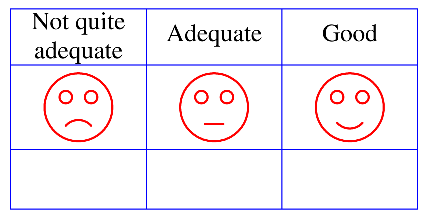
\includegraphics[scale=1.0]{Evurd.pdf}
\end{center}

\newpage

\HRule\\
\textbf{Problem:} \textsc{[MirrorFriendlyMinimumSpanningTree (MFMST)]}\\
\textbf{Input:} An undirected, connected weighted graph $G = (V,E,w)$, where $V = \{1,\dots,n\}$, $E = \{e_1,\dots,e_m\}$ and $w : E \rightarrow \mathbb{N}_0$, and a number $B \in \mathbb{N}$.\\
\textbf{Output:} YES if there is a spanning tree $T \subseteq E$ for $G$ such that
$$max \left\{\nsum\limits_{e_i \in T} w(e_i), \nsum\limits_{e_i \in T} w(e_{m+1-i})\right\} \leq B$$
and NO otherwise.\\
\HRule

\subsection{a) Yeah!}

\subsubsection{Solve an example problem}
\textbf{Input:} $V = \{1,2,3\}$, $E = \{e_1 = \{1,2\},e_2 = \{2,3\},e_3 = \{1,3\}\}$, $w(e_i) = i$ for $i \in \{1,2,3\}$ and $B = 4$.

\end{document}
